\section{Implementación de Encoder.}

\begin{frame}{Prueba de encoder.}
    \begin{columns}[c]
        \column{0.5\textwidth}{
            \begin{figure}[H]
                \centering
                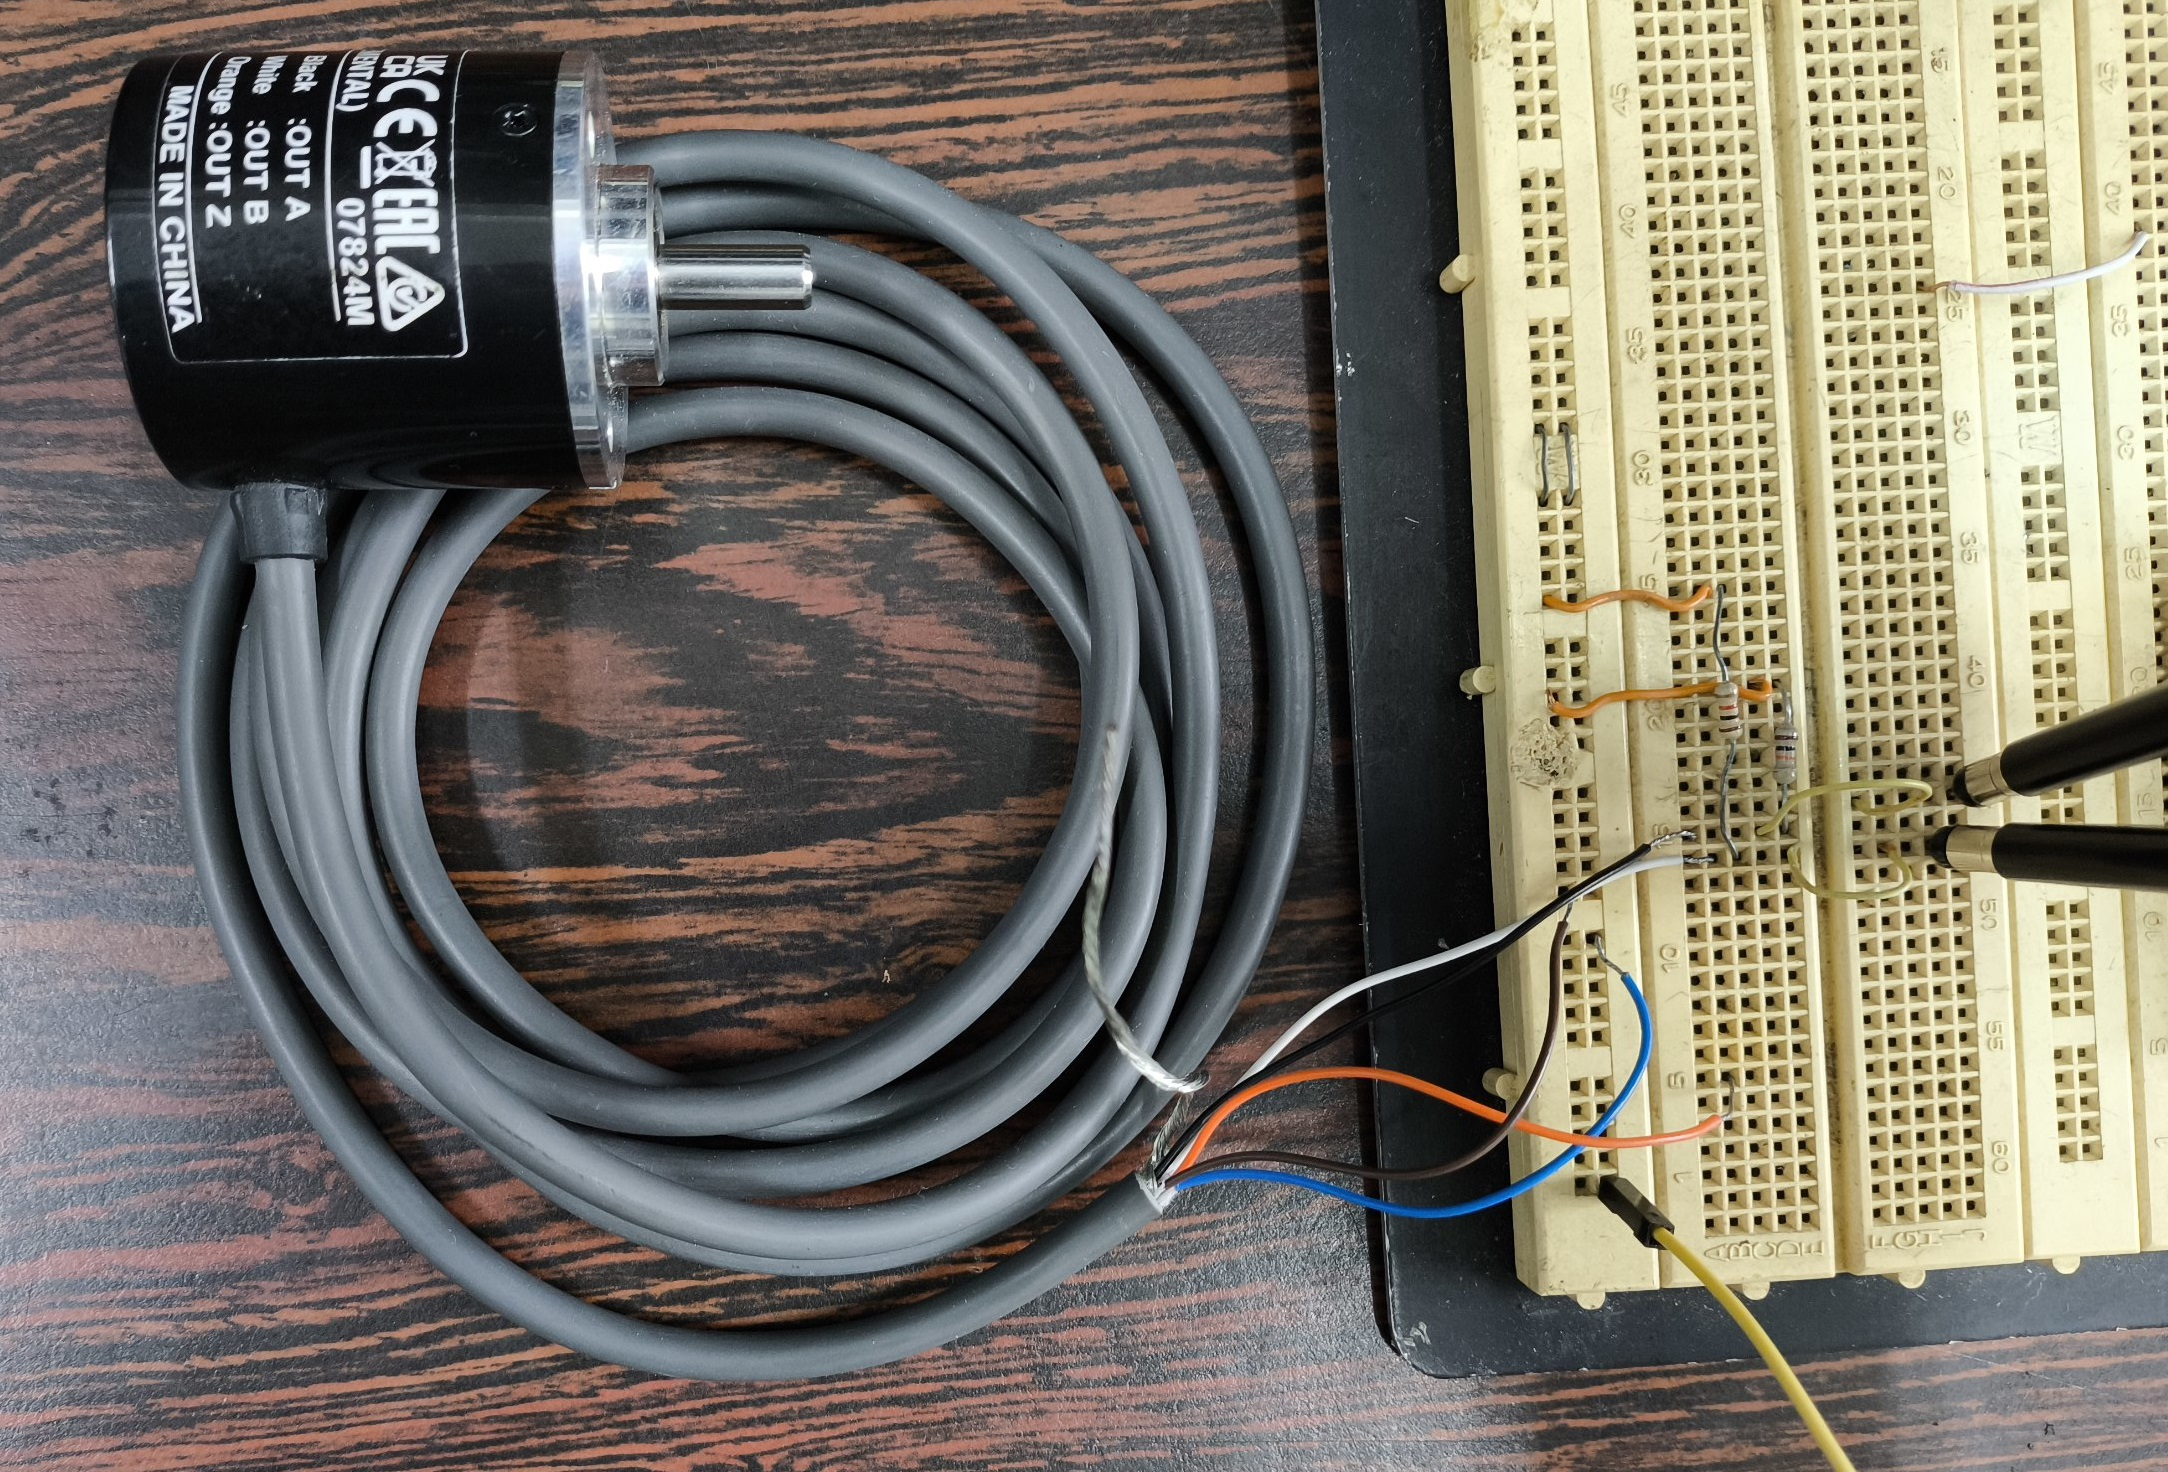
\includegraphics[width=\textwidth]{fig/encoder-prueba.jpg}
                \caption{Montaje para observación y validación del funcionamiento del encoder.}
            \end{figure}
        }
        \column{0.5\textwidth}{
            \begin{figure}[H]
                \centering
                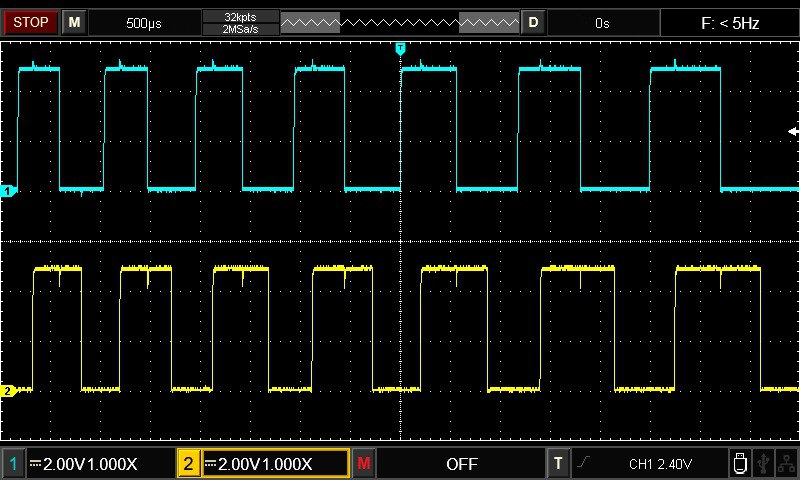
\includegraphics[width=\textwidth]{fig/encoder-senal.jpg}
                \caption{Confirmación de señales recibidas y desfase repectivo de 90°.}
            \end{figure}
        }
    \end{columns}
\end{frame}

\begin{frame}{Libreria de encoder.}
    \begin{columns}[c]
        \column{0.5\textwidth}{
            \begin{figure}[H]
                \centering
                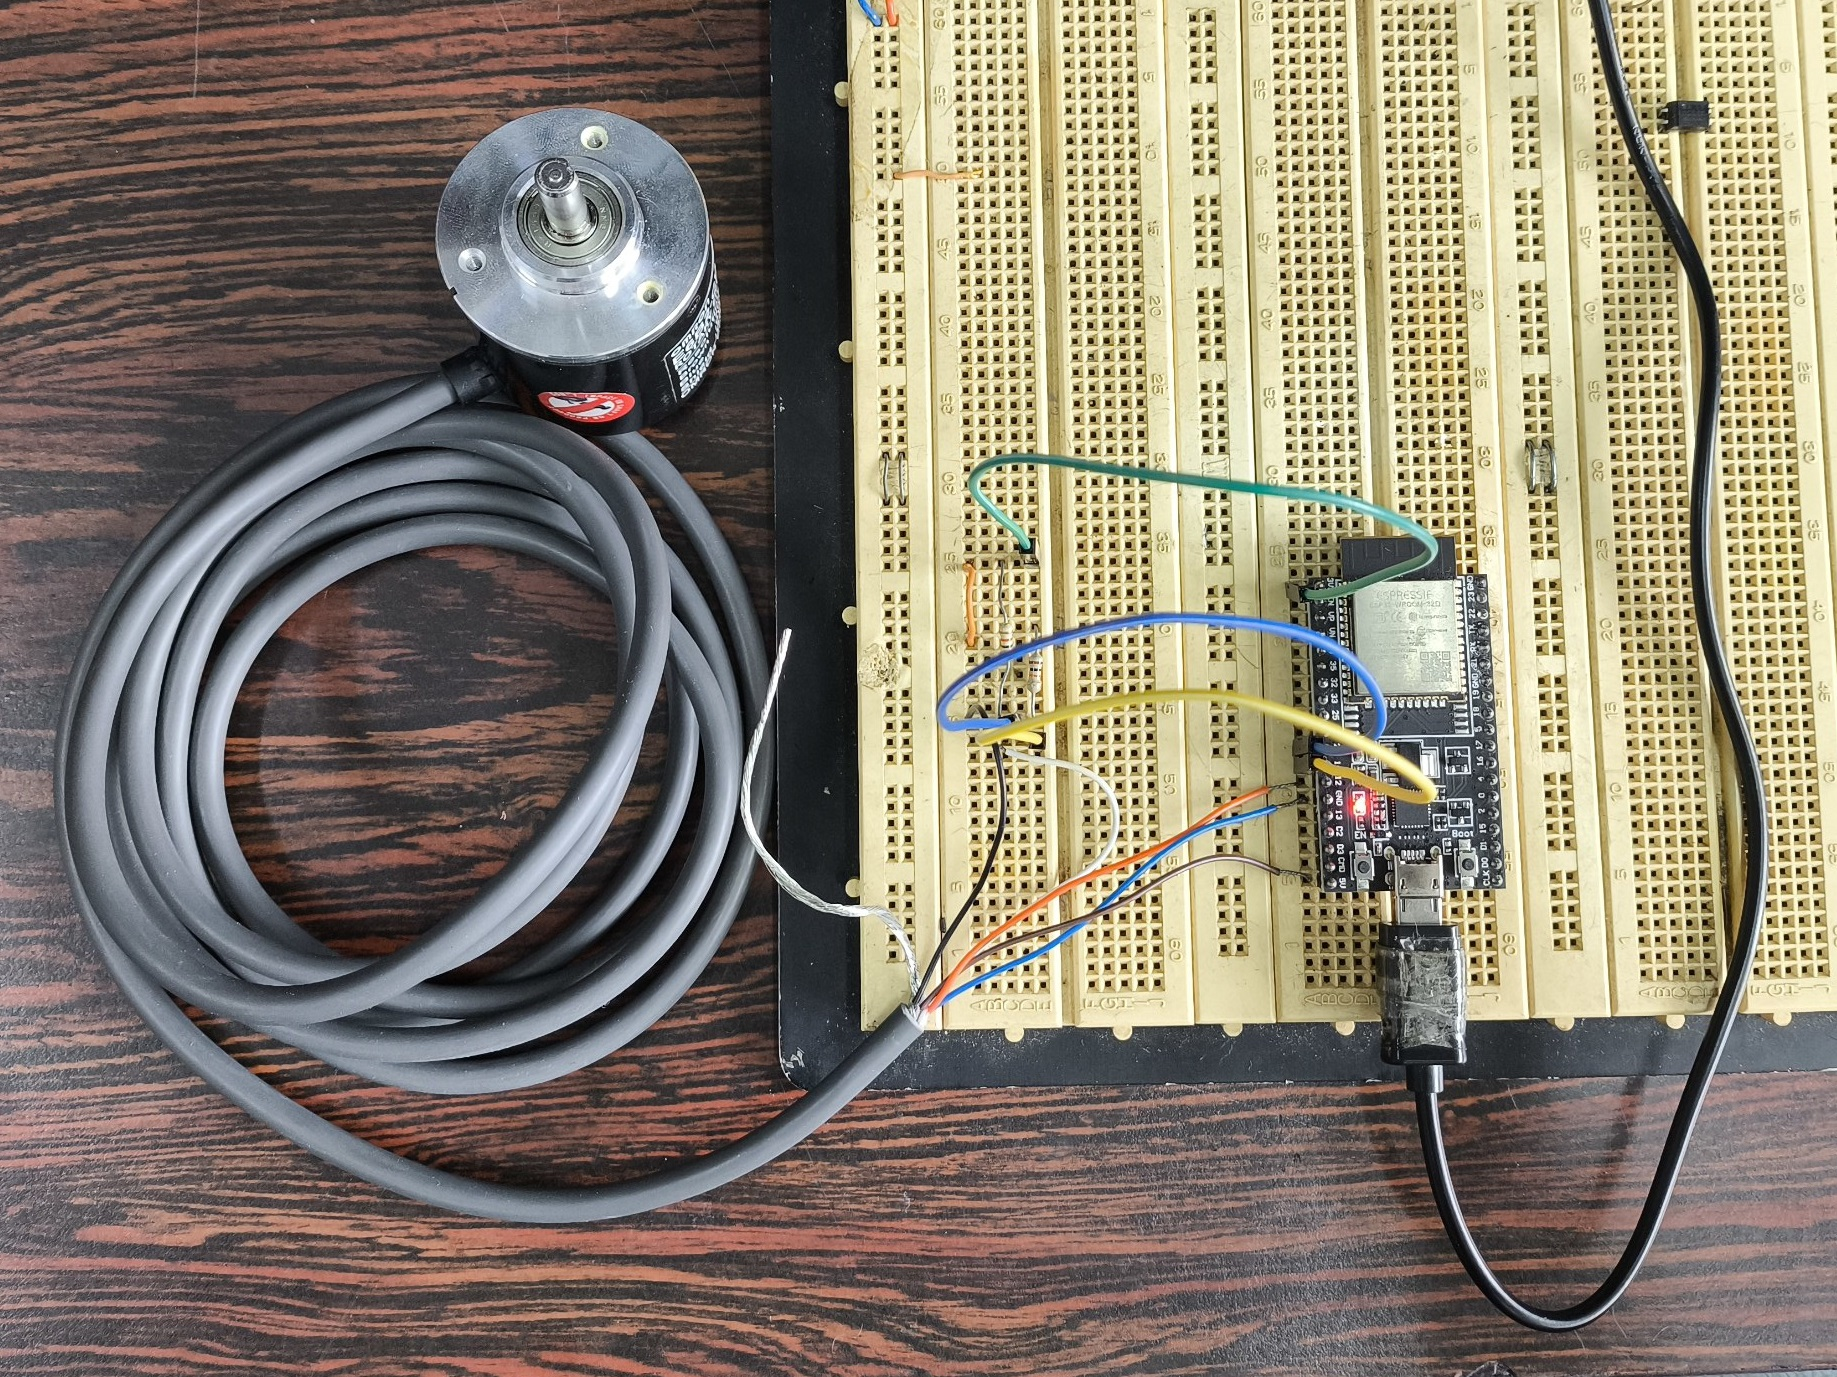
\includegraphics[width=\textwidth]{fig/encoder-esp.jpg}
                \caption{Montaje mínimo para el funcionamiento del encoder y lectura a través del esp32.}
            \end{figure}
        }
        \column{0.5\textwidth}{
            El firmware del ESP32, usando el periférico PCNT, interpreta las señales para calcular el ángulo y detectar el pulso de la fase Z, reseteando el contador. \\
            \begin{figure}[H]
                \centering
                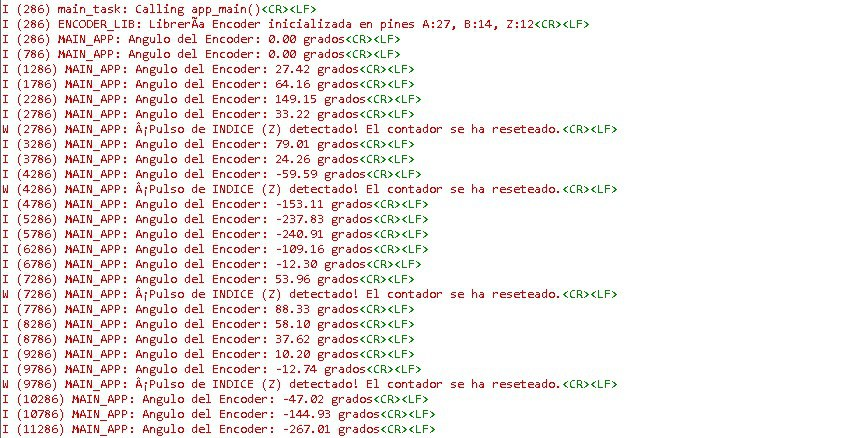
\includegraphics[width=\textwidth]{fig/encoder-code.jpg}
                \caption{Salida serial del codigo respectivo.}
            \end{figure}
        }
    \end{columns}
\end{frame}